\section{Implementation}
\label{sec:implementation}

In this section I will go over the previously discussed modules, and how they are implemented. And why some thing turned out the way they did.

\subsection{The tools}
\label{subsec:the_tools}

Before we look at the implementation, we must first pick our tools. For this particular application I when with Java. Using JavaFX for the user interface and controllers. This meant right from the get go I had cross platform support. A MVC style architecture and with JDBC open access to SQL database connections. The only major issue was speed, as SQLite is known to be fast, whether my application could keep up with the requests that where being performed. However, as SQLite only allows one writer at a time this so was never an issue. The other downside to using Java was not having direct access to the SQLite API through its own interface. But, after looking at the interface everything that i needed was supported through JDBC.

\subsection{The Modules}
\label{subsec:the_modules}

\subsubsection{The view and controller}
\label{subsubsec:imp_veiw}

To begin with we will look at the view, and controllers, as previously mentioned, the architecture is MVC. And we are using JavaFX. JavaFX comes with a whole host of tools for working with the view, and controllers. 
\\\\
Firstly, they have their own file type that is heavily based on HTML, with support for CSS styling. The file can include / imports Java classes into it, allowing for custom items. Each item can be given a unique id that allows it to be controlled with via Java.
\\\\
On the controller side of things, once you are set as the controller for a particular fxml file. The annotation @FXML followed by the type, and unique id, allows Java to inject the item from the fxml file into the variable, giving you full control of it.  
\\\\
The view is made up of four sections, the menu bar, containing the file, edit and other drop downs, including the icons, and tabs. The other three section, represent the left, middle, and right sections of the central pane. This means that any one time i can display three different items. Each of the section have their own fxml file, depending on the situation they may also share a controller. This can be seen below in figure~\ref{fig:view_breakdown}.

\begin{figure}[H]
	\centering
	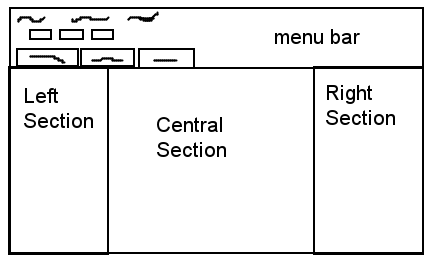
\includegraphics[scale=0.5]{images/view_breakdown.png}
	\caption{View breakdown}
	\label{fig:view_breakdown}
\end{figure}

Looking at the breakdown, you will notice that the menu bar will never change. and should never change as its the navigation used to get around the program. Using this fact the menu bar controller also double up as a 'master' controller. By this I mean it controls what is currently seen in the other three sections. Loading and freeing up to load the necessary sections for that tab. As the central pane is simple split pane, allowing each sections size to be adjusted to fit the users needs. If a section is not needed its just a matter of hiding that panes split bar. 
\\\\
The controllers for each of the sections extend a abstract controller class. The controller class, enforces a model interface object into the constructor. And implements Observer. The model interface allows each controller to separately contact the model, as previously mentioned to collect the data for the view. And by implementing observer we can register our controllers for the signal when the database is updated. Meaning we can collect the updated information as soon as it's ready. Without having to wait, or having a manual refresh button.    

\subsubsection{Model interface}
\label{subsubsec:imp_model_interface}

The model interface is how the controllers contact the other sub modules. Its a repository design, that helps keep everything de-coupled, with the exception of the Live updater. All modules including the model interface implement their representing interface. Allowing the implementation to change while keeping the same external view. This enables the design to be adapted to other systems other then SQLite. Below figure~\ref{fig:model_interface_design} show the layout of the model interface.

\begin{figure}[H]
	\centering
	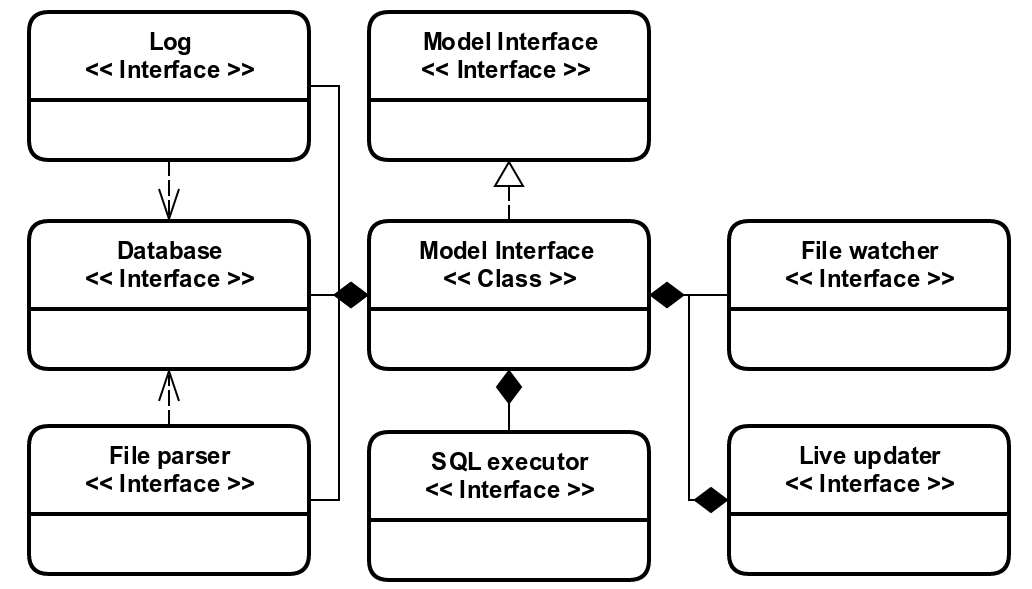
\includegraphics[scale=0.3]{images/model_interface_design.png}
	\caption{Model interface}
	\label{fig:model_interface_design}
\end{figure}

As you can see everything is attached to the model interface, and only the live updater is the exception with a copy of the model. In addition to provide access to the other modules, it has a very small amount of implementation, that is only used when every module is affected. Such as the case of setting up, closing and opening a database, which are all calls to the corresponding method on the modules interfaces. 

\subsubsection{The database}
\label{subsubsec:databse_imp}

The database module is made up of two parts, the interface and the storage. The interface is what everything else has access to allowing it to control the storage without interference. The storage is made up of database items, that contain a "snapshot" of the current state of the database file.
\\\\
The interface allows adding of new database items, retrieving of database items and stepping through the time line of database objects. And complete clearing of database items, used with setting up and opening a new database, in order to make sure that the items are not mixed up with the different files.
\\\\
The database items in the storage, are a data structure, made of two parts the meta-data, and B-Tree. The meta-data contains all the information in the header, including a few others such as number of tables, file name, and more. The B-Tree is a custom implementation, holding the various B-Tree pages, as represented in the file. The database items are filled with information via the file parser. Out of all the classes, the database items, are the most used, being sent to the view for displaying, and modified by the various other modules during creation. 

\subsubsection{File watcher}
\label{subsubsec:file_watcher_imp}

In order to workout when the database was updated, to collect live data. I had two options, use SQLites API or watch the file. The API provided by SQLite is on a per connection base meaning that I would only revive signals when my own application sent of SQL commands, which are of no use to me, as  I already know when the commands a sent out. This left me with the latter option, watching the file. Since SQLite is a single file, every time the file / database was updated so would the last modified time. In addition to this as SQLite only allows one writer at a time, I would revive a signal every update consistently.  
\\\\
The original implementation utilised Java's WatchService api. However, when I used it, I found it to be hit or miss whether it would register the change. And at one point failed to detect any changes. So i ended up rolling my own solution, which is a simple while true loop, recorded the last modified time, then when the time differs we send out a single to the rest of the application. 
\\\\
Due to the polling nature of this module, it runs inside its own thread, and communicates over an observer patten, that any another class can tune into, providing they implement the Observer interface. This meant that the thread could process the updated databases without stopping or slowing down the user interface and other interactions.

\subsubsection{File parser}
\label{subsubsec:file_parser_imp}

The file parser does exactly what it says on the tin, it takes a database file, a database object, and converts the file into the object. Parsing the database, started off with the, checking the magic number, then the header, before moving onto the pages. The magic number and header information where all about reading the first 100 bytes, correctly. For the pages I relied heavily upon recursion.
\\\\
First I would parse the page header, then switch into the method, that dealt with that type of page, who would then call the original method, when it reached a page number.  Each page was represented as a different node. As the recursive method returned a node, representing that node, and all of its children, left a elegant and effective design, unless we run out of stack with a huge database. Below is the psudocode of the algorithm:

\begin{lstlisting}	
public void parseBTree(stream, database) {
	database.getBTree().setRoot(parsePage(stream, 1, 
								database.getPageSize()));
}

public Node parsePage(stream, pageNumber, pageSize) {
	Node node = new Node();
	PageHeader header = parseHeader(stream, pageNumber, pageSize);
	
	BTreeCell cell;
	switch(header.getType()) {
		case (TABLE_BTREE_LEAF_CELL) {
			cell = parseTableBtreeLeafCell(stream, pageNumber, 
											pageSize);
		}
		....
	}
	if (header.getType() == INTERIOR_CELL) {
		node.addChild(parsePage(in, pageHeader.getRightMostPointer(), 
						pageSize));
	}
	node.setData(cell);
	return node;
}

public cell parseTableBtreeLeafCell(InputStream, PageHeader, Node) {
	Cell cell = new Cell();
	
	int cellPointers[] = header.getCellPointers();
	foreach(cellpointer) {
		cell.data = readData();		
		if (cell has pageNumber) {
			node.addChild(parsePage(in, pagenumber, 
						pageSize));
		}
	}
	
	return cell;
}
\end{lstlisting}

While that solves how to go about parsing the tree, one major problem was decoding the 'varints' mentioned in section~\ref{subsubsec:sqlite_data_encoding} especially as we needed to count the number of bytes for the record headers. Below shows the psudocode algorithm that I made in order to decrypt them: 

\begin{lstlisting}	
private long[] decodeVarint(stream) {
	long[] value = new long[];
	byte[] varint = new varint[9];
	
	for (i = 0 to 9) {
		varint[i] = stream.readByte();
		if (first bit is not set) {
			break;
		}
	}
	
	if (i == 0) {
		value[0] = 0;
		value[1] = 1;
	} else {
		for (j == 0 to i) {
			varint[j] = (varint[j] << 1);
		}
		value[0] = varint.toLong();
		value[1] = i + 1;
	}
	return value;
}
\end{lstlisting}

The first value returned is the value of the varint, and the second its size. Now we have that all sorted decoding the record headers, and other section of the file is easy.

\subsubsection{The log}
\label{subsubsec:log_imp}

The log, as briefly mentioned in the design section, had a complete change compared to the original plan. The original plan was to have the log run on its own without having to relay on other modules, and would retrieve the original SQL commands that where sent to it. While looking at SQLite there were three ways I could have done it in addition to my final implementation.
\\\\
The first technique I looked at utilised SQLites triggers. Triggers execute SQL commands when, a Delete, insert or update is performed on a table, with a optional where clause. Using this \cite{sqlitetriggers} used three separate triggers to long the time, changes before and after, and type of action performed on the table. The last part is one of the reason why I went for another technique. Firstly, I would need to have three triggers per table in the database, so N*3 triggers where N is the number of tables. Secondly, in order to accomplish this, I needed my own table that it changes where the changes are stored to, hence the log file in my original design, where i would attach to the database and write to it. lastly, the triggers mean altering the database file, this is something I wanted to avoid as much as possible.  
\\\\
The second solution, was to try and hook into SQLite through its API more specifically the sqlite3\verb|_|trace function. You pass it a callback function, that is called with the SQL commands, at various stages as it passes through the system. Unfortunately for me at the current time the JBDC for SQLite did not support the function that I needed. So I ended up writing a couple C functions that I could then call from Java in order to access the functions. It worked for the most part, apart from that method only calls the callback function for SQL sent from the current application. Which is useless to me as I wanted to see all the changes. 
\\\\
So with two ways down the third way was to write my own extension to SQLite, or download the source code, and modify to suit my needs it. The seemed to be way to far from the original path, and if I used a custom version it means that it would be limited to only my version of SQLite. And as mentioned previously, I wanted to not modify the data if possible, so writing an extension, that would have to be loaded into SQLite and attached to the database, possibly conflicting with any other extensions they might have left me with my final option.
\\\\
The final option, while less sophisticated then the others, works well, although I do not get the original requests. I do end up recording the time, and all changes that happened per command. Since the database storage contains all of the previous versions like a snapshot of the database. when a update comes in I simply compare the new updated database to the last database that passed through the application.
\\\\
In order to compare database though required looping through every data value in both trees and comparing them, not only the data vale, but also the added pages and removal of pages. This could not be detected through any of the other techniques. Clearly looping through every single item in a larger database would quickly become a bottleneck, and slow the application and parsing down. So in order to speed it up, I did two things, firstly hashed the data array, If the hashes matched then we do not have to loop through the data. the second this was to adjusted my B-trees into a modified version of the Merkle Tree patented by \cite{merkletree}. The basic idea behind the merkle tree is that each node in the tree has a hash of its childrens hash, all the way down to the leaf node, who hash is based on the contents. Below figure~\ref{fig:merkle_tree} shows a digram of the merkle tree.

\begin{figure}[H]
	\centering
	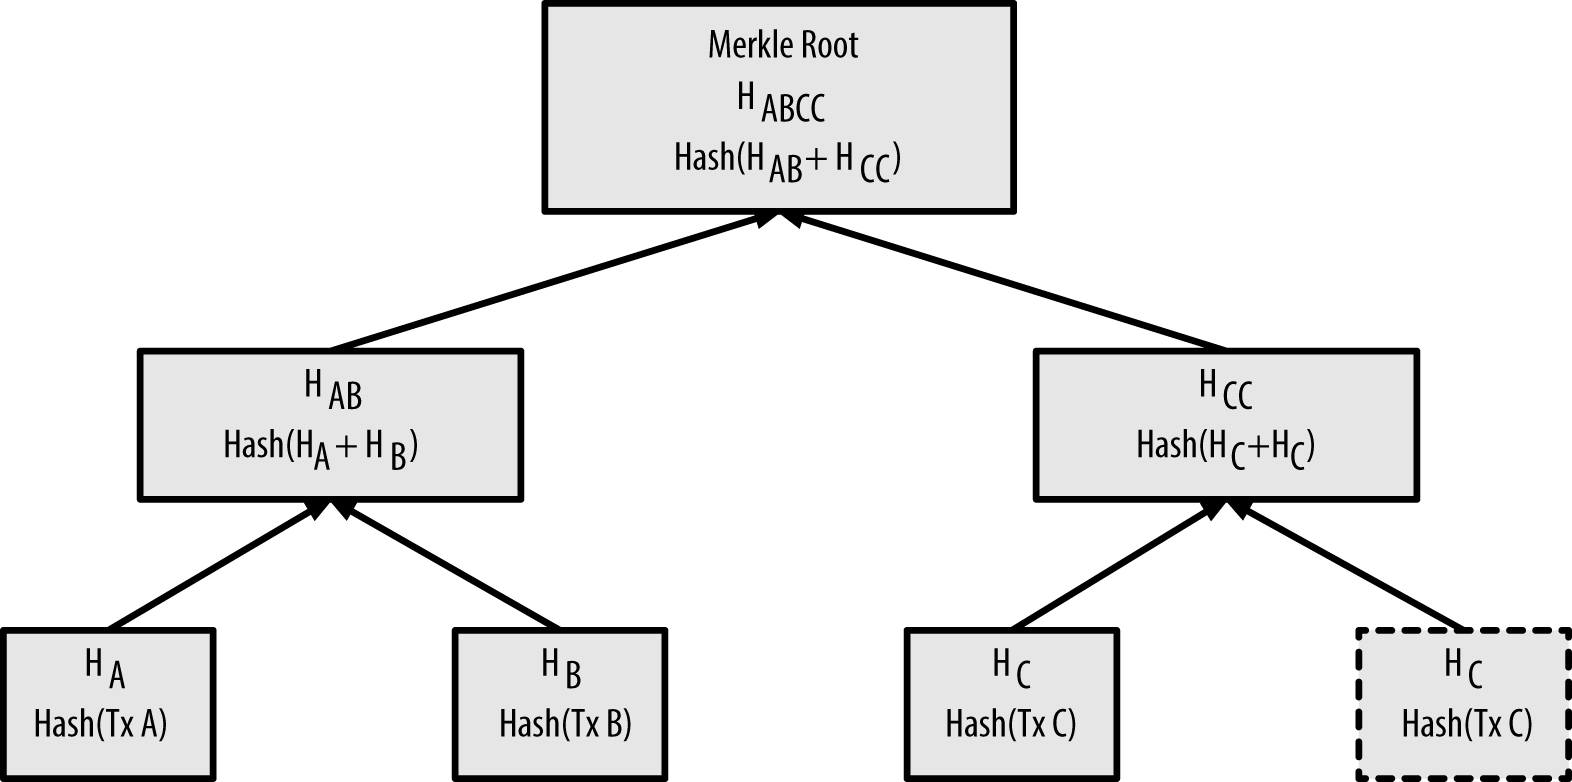
\includegraphics[scale=1.0]{images/merkle_tree.png}
	\caption{Node hashes in a  merkle tree \citep{bitcoin}}
	\label{fig:merkle_tree}
\end{figure}

This means we can tell if there is any change in the current section tree just by comparing the nodes hashes without having to loop over them. meaning that we will only loop over the tree at all when a change is seen. otherwise we can skip it. Creating an unnoticeable change unless many nodes are changed at once. The hash for node is calculated off the hash of the data and number of children meaning we will also know if a page has been added or removed. 

\subsubsection{Live Updater}
\label{subsubsec:live_Updater_imp}

The Live updater...

\subsubsection{SQL executor}
\label{subsubsec:sql_executor_imp}

The SQL executor...